% Copyright 2004 by Till Tantau <tantau@users.sourceforge.net>.
%
% In principle, this file can be redistributed and/or modified under
% the terms of the GNU Public License, version 2.
%
% However, this file is supposed to be a template to be modified
% for your own needs. For this reason, if you use this file as a
% template and not specifically distribute it as part of a another
% package/program, I grant the extra permission to freely copy and
% modify this file as you see fit and even to delete this copyright
% notice. 

\documentclass{beamer}
\usepackage{algorithm2e}
\usepackage{amsmath}
\usepackage{graphicx}
\usepackage{subcaption}

% There are many different themes available for Beamer. A comprehensive
% list with examples is given here:
% http://deic.uab.es/~iblanes/beamer_gallery/index_by_theme.html
% You can uncomment the themes below if you would like to use a different
% one:
%\usetheme{AnnArbor}
%\usetheme{Antibes}
%\usetheme{Bergen}
%\usetheme{Berkeley}
%\usetheme{Berlin}
%\usetheme{Boadilla}
%\usetheme{boxes}
%\usetheme{CambridgeUS}
%\usetheme{Copenhagen}
%\usetheme{Darmstadt}
%\usetheme{default}
%\usetheme{Frankfurt}
%\usetheme{Goettingen}
%\usetheme{Hannover}
%\usetheme{Ilmenau}
%\usetheme{JuanLesPins}
%\usetheme{Luebeck}
\usetheme{Madrid}
%\usetheme{Malmoe}
%\usetheme{Marburg}
%\usetheme{Montpellier}
%\usetheme{PaloAlto}
%\usetheme{Pittsburgh}
%\usetheme{Rochester}
%\usetheme{Singapore}
%\usetheme{Szeged}
%\usetheme{Warsaw}

\title{Deep Contact}

% A subtitle is optional and this may be deleted
\subtitle{Accelerating Rigid Simulation with Convolutional Networks}

\author{J.~Wu}
% - Give the names in the same order as the appear in the paper.
% - Use the \inst{?} command only if the authors have different
%   affiliation.

\institute[University of Copenhagen] % (optional, but mostly needed)
{
  Department of Computer Science\\
  University of Copenhagen
}
% - Use the \inst command only if there are several affiliations.
% - Keep it simple, no one is interested in your street address.

\date{Master Thesis Defense, 2018}
% - Either use conference name or its abbreviation.
% - Not really informative to the audience, more for people (including
%   yourself) who are reading the slides online

\subject{Theoretical Computer Science}
% This is only inserted into the PDF information catalog. Can be left
% out. 

% If you have a file called "university-logo-filename.xxx", where xxx
% is a graphic format that can be processed by latex or pdflatex,
% resp., then you can add a logo as follows:

% \pgfdeclareimage[height=0.5cm]{university-logo}{university-logo-filename}
% \logo{\pgfuseimage{university-logo}}

% Delete this, if you do not want the table of contents to pop up at
% the beginning of each subsection:
\AtBeginSubsection[]
{
  \begin{frame}<beamer>{Outline}
    \tableofcontents[currentsection,currentsubsection]
  \end{frame}
}

% Let's get started
\begin{document}

\begin{frame}
  \titlepage
\end{frame}

\begin{frame}{Outline}
  \tableofcontents
  % You might wish to add the option [pausesections]
\end{frame}

% Section and subsections will appear in the presentation overview
% and table of contents.
\section{Introduction}

\subsection{Previous Work}

\begin{frame}{Previous Work}
  \begin{itemize}
  \item {
    My first point.
  }
  \item {
    My second point.
  }
  \end{itemize}
\end{frame}

\subsection{Thesis Overview}

% You can reveal the parts of a slide one at a time
% with the \pause command:
\begin{frame}{Thesis Overview}
%  \begin{itemize}
%  \item {
%    Modeling Contact.
%    \pause % The slide will pause after showing the first item
%  }
%  \item {   
%    Second item.
%  }
%  % You can also specify when the content should appear
%  % by using <n->:
%  \item<3-> {
%    Third item.
%  }
%  \item<4-> {
%    Fourth item.
%  }
%  % or you can use the \uncover command to reveal general
%  % content (not just \items):
%  \item<5-> {
%    Fifth item. \uncover<6->{Extra text in the fifth item.}
%  }
%  \end{itemize}
\end{frame}

\section{Particles-Grid-Particles}

\subsection{Grid-Particle Method}
\begin{frame}{Grid-Particle Method}
In order to generate accessible data for CNN model, we transform every state into a set of grid images.
\begin{itemize}
\item {It can make the simulation states be expressed by a set of matrixes, which can be accessible for deep neural networks.
    \pause
}
\item {}
\end{itemize}
\end{frame}
\begin{frame}{Grid-Particle Method}{Workflow}
The whole workflow can be described as,
\begin{enumerate}
\item {
Based on Smoothed Particle Hydrodynamics(SPH), map current state(\(m, v_x, v_y, \omega, n_x\)) to a image(the number of channel is 5.), which is called feature image.
\pause
}
\item {
The feature image will be used as input to a model(created by a convolutional neural network), then one image(the number of channels is 2) will be getting, which can be called label image.
\pause
}
\item {
For all contacts positions, interpolated values will be gener- ated based on label image. Then, the values will be used as starting iterate values for contact force solver. In our hypoth- esis, the given starting values will speed up the solver to reach convergence.
}

\end{enumerate}
\end{frame}
\subsection{Smoothed Particle Hydrodynamics}

\begin{frame}{Smoothed Particle Hydrodynamics}{Fundamentals}
The heart of SPH is a kernel interpolation method which allows any function to be expressed in terms of its values at a set of disordered points - the particles.
\pause
\begin{equation}
        A_{I}(\textbf{r}) = \int A({\textbf{r}}^{\prime})W(\|\textbf{r} - \textbf{r}^{\prime}\|, h)\mathrm{d}\textbf{r}^{\prime}
\end{equation}
\pause
where the integration is over the entire space, and $W$ is an in-
terpolating kernel with
\pause
\begin{equation}
        \int W(\|\textbf{r} - \textbf{r}^{\prime}\|, h)\mathrm{d} \textbf{r}^{\prime} = 1
\end{equation}
For numerical work,
\pause
\begin{equation}
        A_{S}(\textbf{x}) = \sum_{i}A(\textbf{x}_{i})W(\|\textbf{x}_{i}-\textbf{x}\|, h)
\end{equation}

\end{frame}
\begin{frame}{Smoothed Particle Hydrodynamics}{Kernels}
\begin{itemize}
\item {
\textbf{Poly6}
\pause
\begin{equation}
        W_{poly 6}(\textbf{r}, h) = \frac{315}{64\pi h^{9}}
            \begin{cases}
                (h^2 - \|\textbf{r}\|^2)^3 & 0 \le \|\textbf{r}\| \le h \\
                0 & \textrm{Otherwise}
            \end{cases}
\end{equation}
\pause
}
\item {
\textbf{Spicky}
\pause
\begin{equation}
        W_{spiky}(\textbf{r}, h) = \frac{15}{\pi h^6}
            \begin{cases}
                (h - \|\textbf{r}\|)^3 & 0\le\|\textbf{r}\|\le h \\
                0 & \textrm{Otherwise}\\
            \end{cases}
\end{equation}
}
\end{itemize}
\end{frame}

\begin{frame}{Smoothed Particle Hydrodynamics}{Kernels}
\begin{figure}
        \centering
        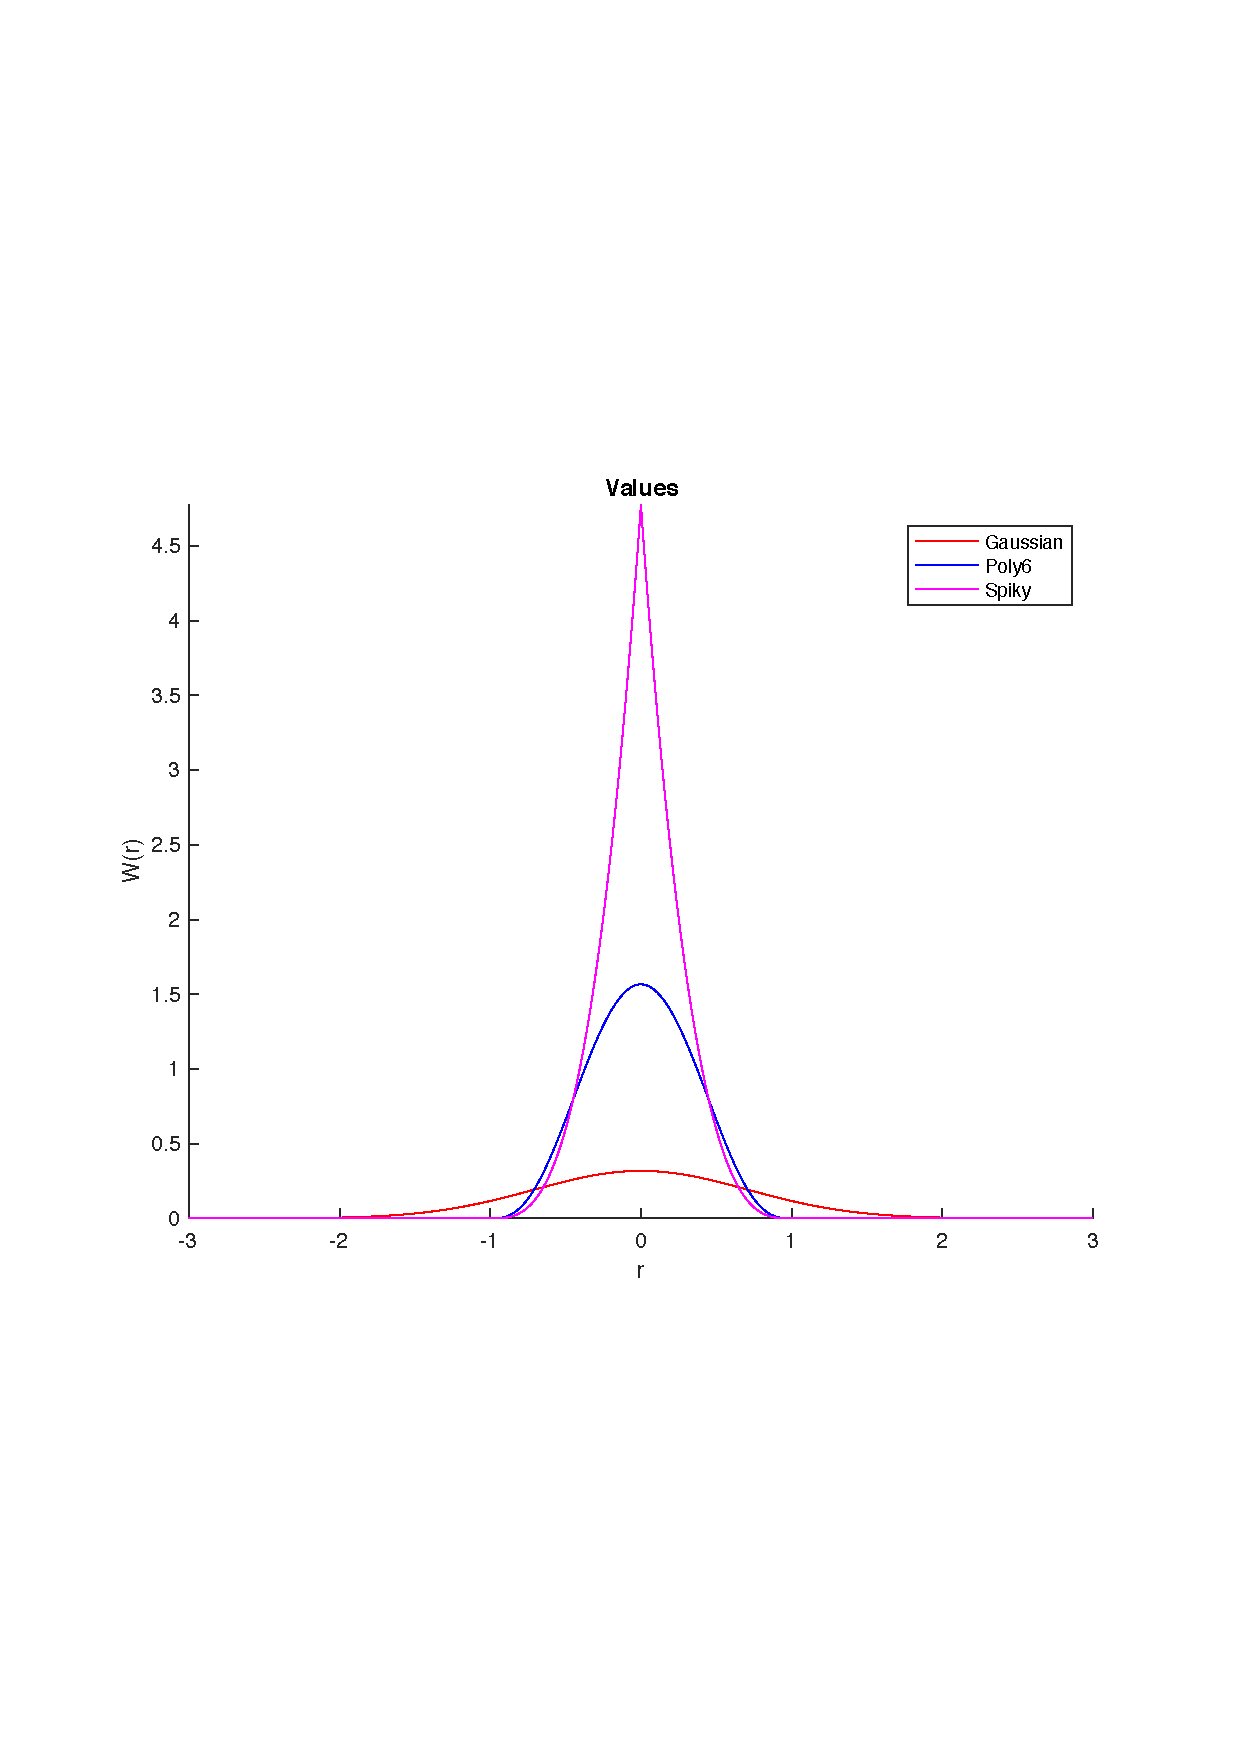
\includegraphics[scale = 0.3]{../report/Figures/kernels}
        \caption{Comparation of different kernels, we set smoothing length $h = 1$ here.}
\end{figure}
\end{frame}

\begin{frame}{Smoothed Particle Hydrodynamics}{Kernels}
\begin{figure}
        \centering
        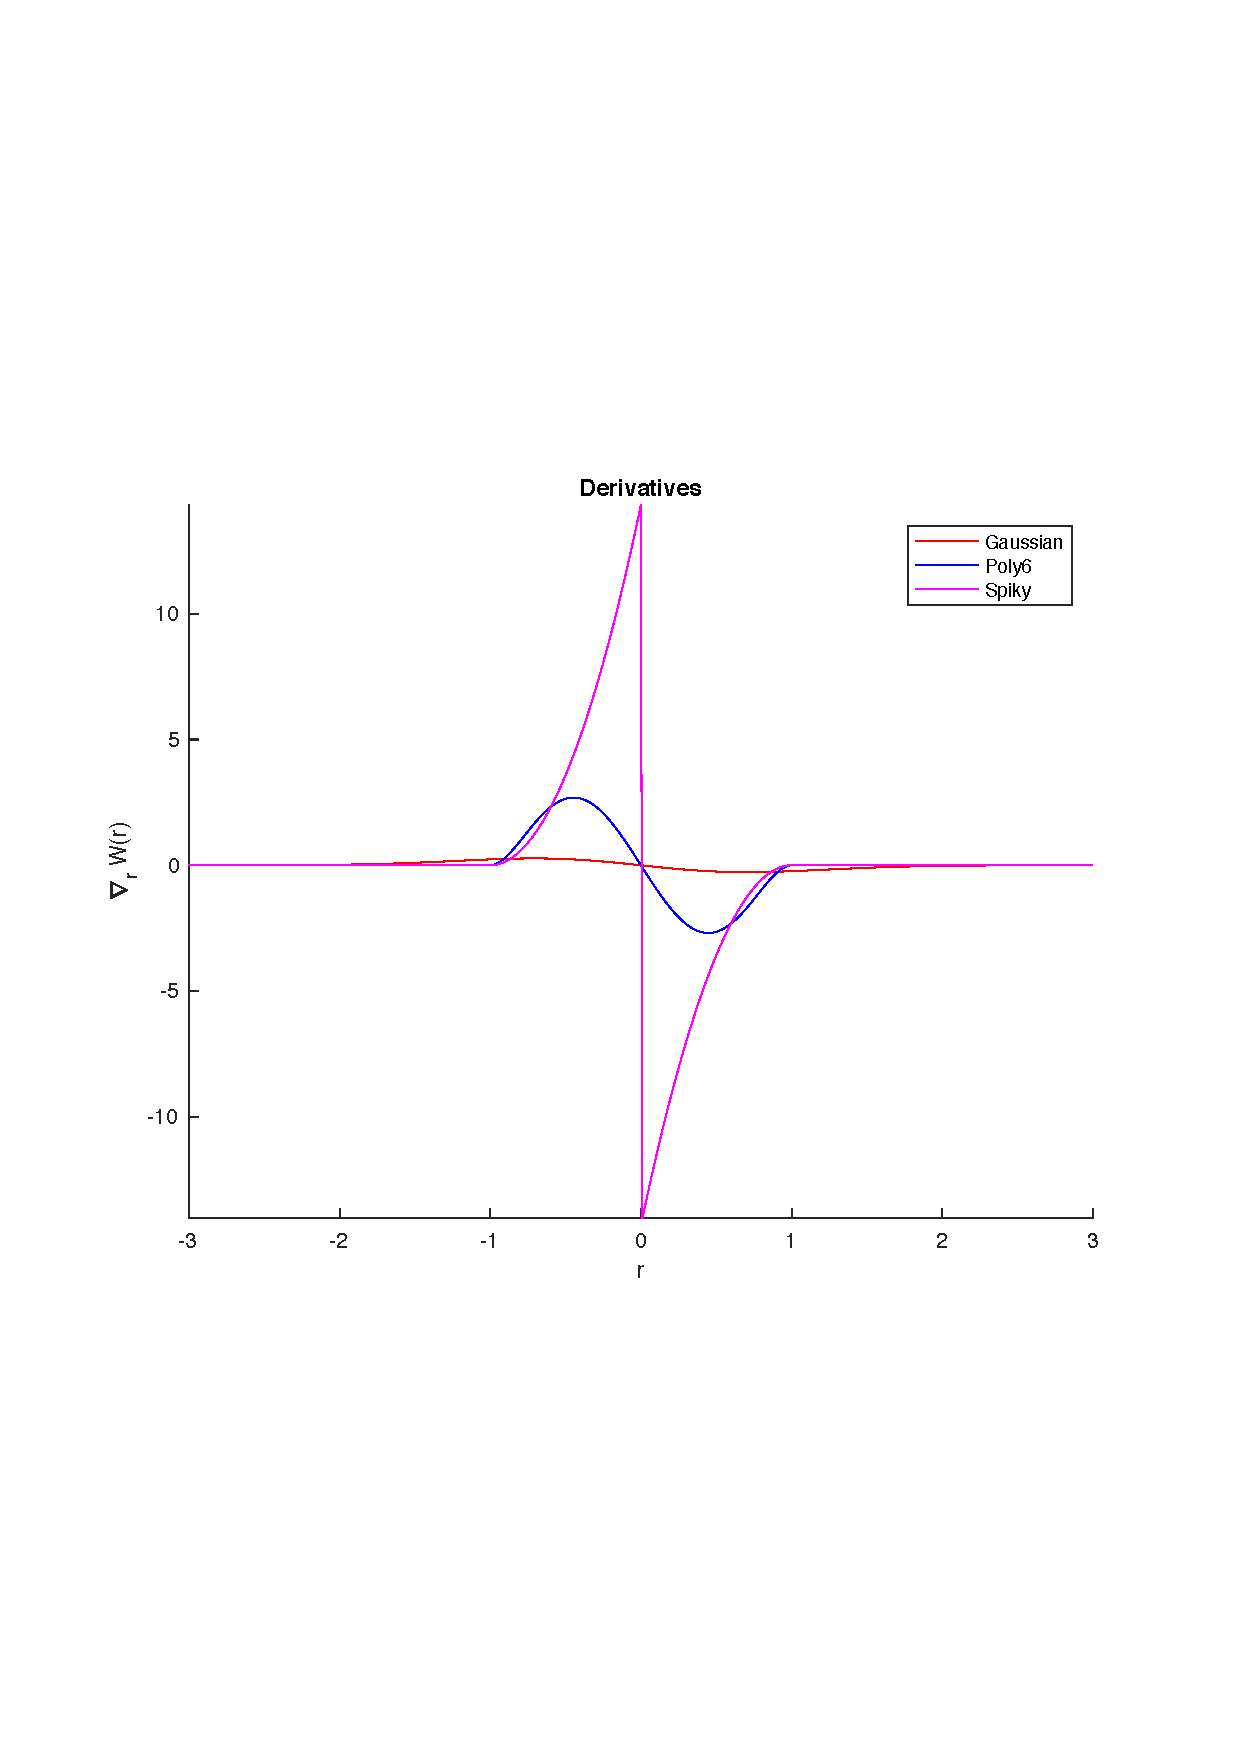
\includegraphics[scale = 0.3]{../report/Figures/kenels_de}
        \caption{Comparation of gradient of different kernels, we set $h = 1$ here. }
\end{figure}
\end{frame}

\begin{frame}
%\begin{algorithm}
%        \KwData{Given a set of contacts $\mathcal{C}$ between a set of bodies $\mathcal{B}$ and the state in time $t$, as well as all the spacial positions of grid nodes $\mathbf{x}$}
%        \KwResult{the contact grid image $\pmb{G}_{\lambda}$}
%        \For{all $i$ and $j$}{
%            1. Find the nearest neihbors $\mathcal{C}_{near} \subseteq \mathcal{C}$ around $\mathbf{x}_{ij}$ \\
%            2. read the current contact forces values and its position.
%                $$\pmb{q}_k, \pmb{\lambda}_{k}~~k\in\mathcal{C}_{near}~~\pmb{\lambda} = [\lambda_n, \lambda_t]$$ \\
%            3. Compute grid values
%                $$\pmb{G}_{\lambda}(i, j) \gets \sum_{k\in \mathcal{C}_{near}}W(\mathbf{x}_{ij}, \pmb{q}_{k})\pmb{\lambda}_k$$
%        }
%        \caption{Mapping contacts into a grid image. It can be called by $Contacts2grid(\mathbf{x}, \mathcal{C})$}
%\end{algorithm}
\end{frame}

\subsection{Bilinear Interpolation}
\begin{frame}{Bilinear Interpolation}
Once getting contact grid image, we need transform the grid image to a physical state, specific contact values in each contact point. We applied bilinear interpolation in our case.
\pause
\begin{figure}
        \centering
        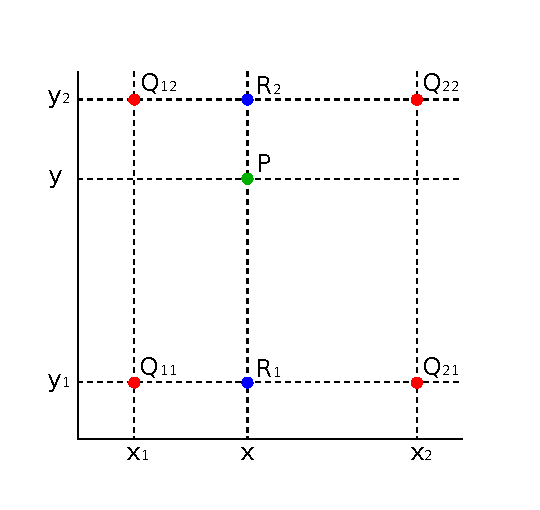
\includegraphics[scale = 0.5]{../report/Figures/inp}
        \caption{The figure shows the visualization of bilinear interpolation. The four red dots show the data points and the green dot is the point at which we want to interpolate.}
\end{figure}
\end{frame}

\begin{frame}{Bilinear}
we can firstly do linear interpolation in the $x$-direction. This yields
\pause
\begin{subequations}
        \begin{align}
            f(x,y_{1})&\approx {\frac {x_{2}-x}{x_{2}-x_{1}}}f(Q_{11})+{\frac {x-x_{1}}{x_{2}-x_{1}}}f(Q_{21}),\\
            f(x,y_{2})&\approx {\frac {x_{2}-x}{x_{2}-x_{1}}}f(Q_{12})+{\frac {x-x_{1}}{x_{2}-x_{1}}}f(Q_{22}).
        \end{align}
        \label{eq:2}
\end{subequations}
\pause
After getting the two values in $x-$direction $f(x, y_1)$ and $f(x, y_2)$, we can combine these values to do interpolation in $y-$ direction.
\pause
\begin{equation}
        f(x,y) \approx {\frac {y_{2}-y}{y_{2}-y_{1}}}f(x,y_{1})+{\frac {y-y_{1}}{y_{2}-y_{1}}}f(x,y_{2})
    \end{equation}
\end{frame}

\begin{frame}{SPH method}{Experiments}
\begin{figure}[!h]
        \centering
        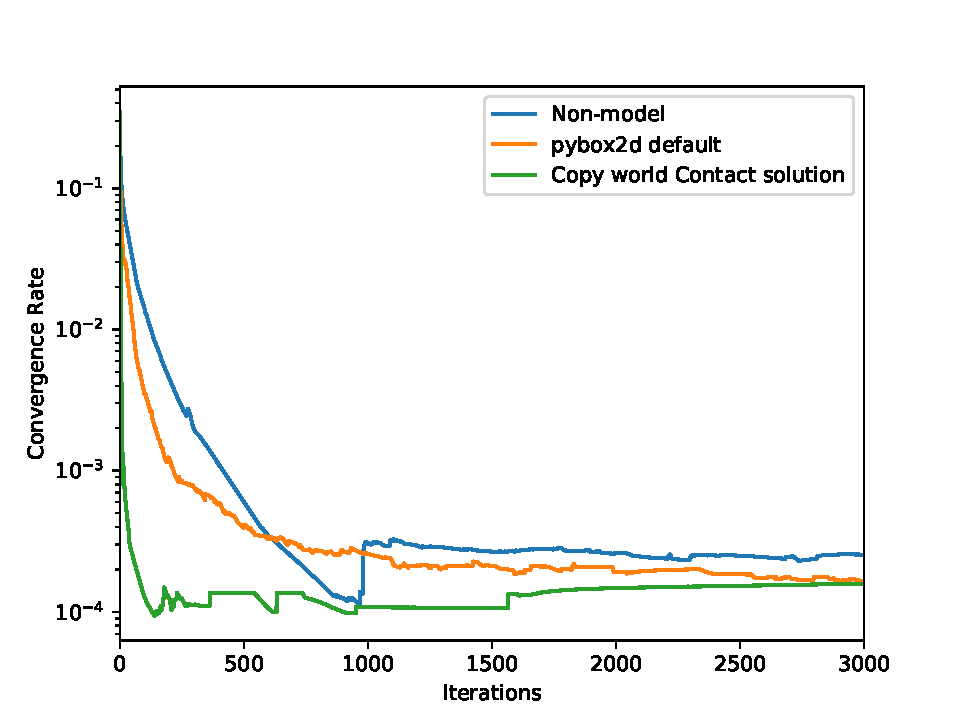
\includegraphics[scale = 0.4]{../report/Figures/nosph}
        \caption{Average convergence rate for different models(not including \textbf{SPH-based model}).}
        \label{fg:nosph}
\end{figure}
\end{frame}
\begin{frame}{SPH method}{Experiments}
\begin{figure}[!h]
        \centering
        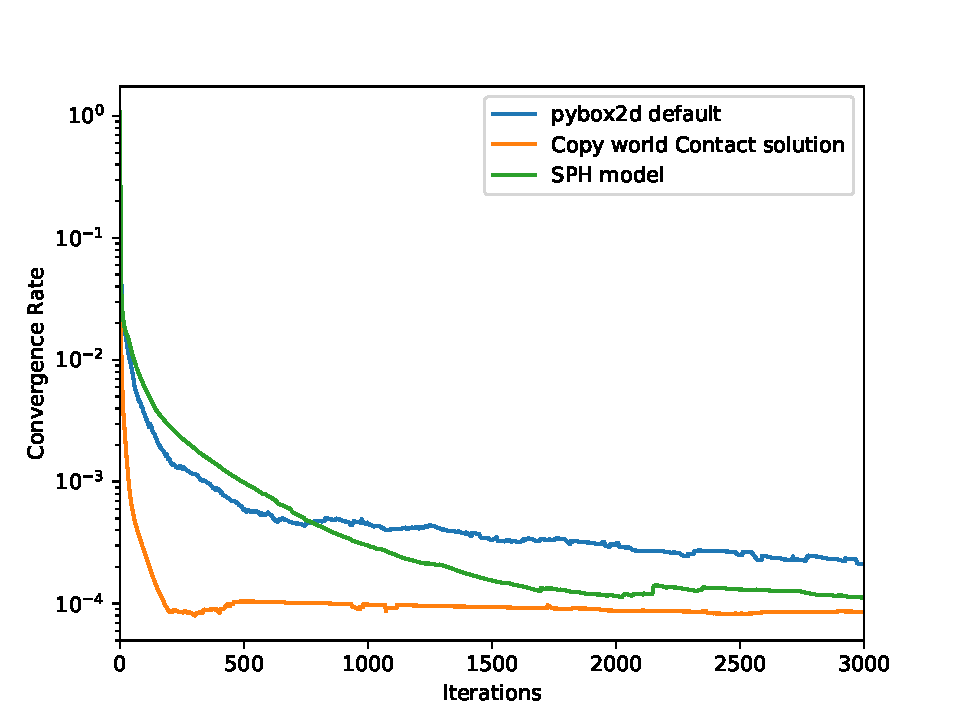
\includegraphics[scale = 0.4]{../report/Figures/addsph}
        \caption{Average convergence rate for different models(not including \textbf{SPH-based model}).}
        \label{fg:nosph}
\end{figure}
\end{frame}

\section{Deep Learning Model}
\subsection{CNN Architecture}
\begin{frame}{CNN Architecture}
\begin{figure}[!h]
        \centering
        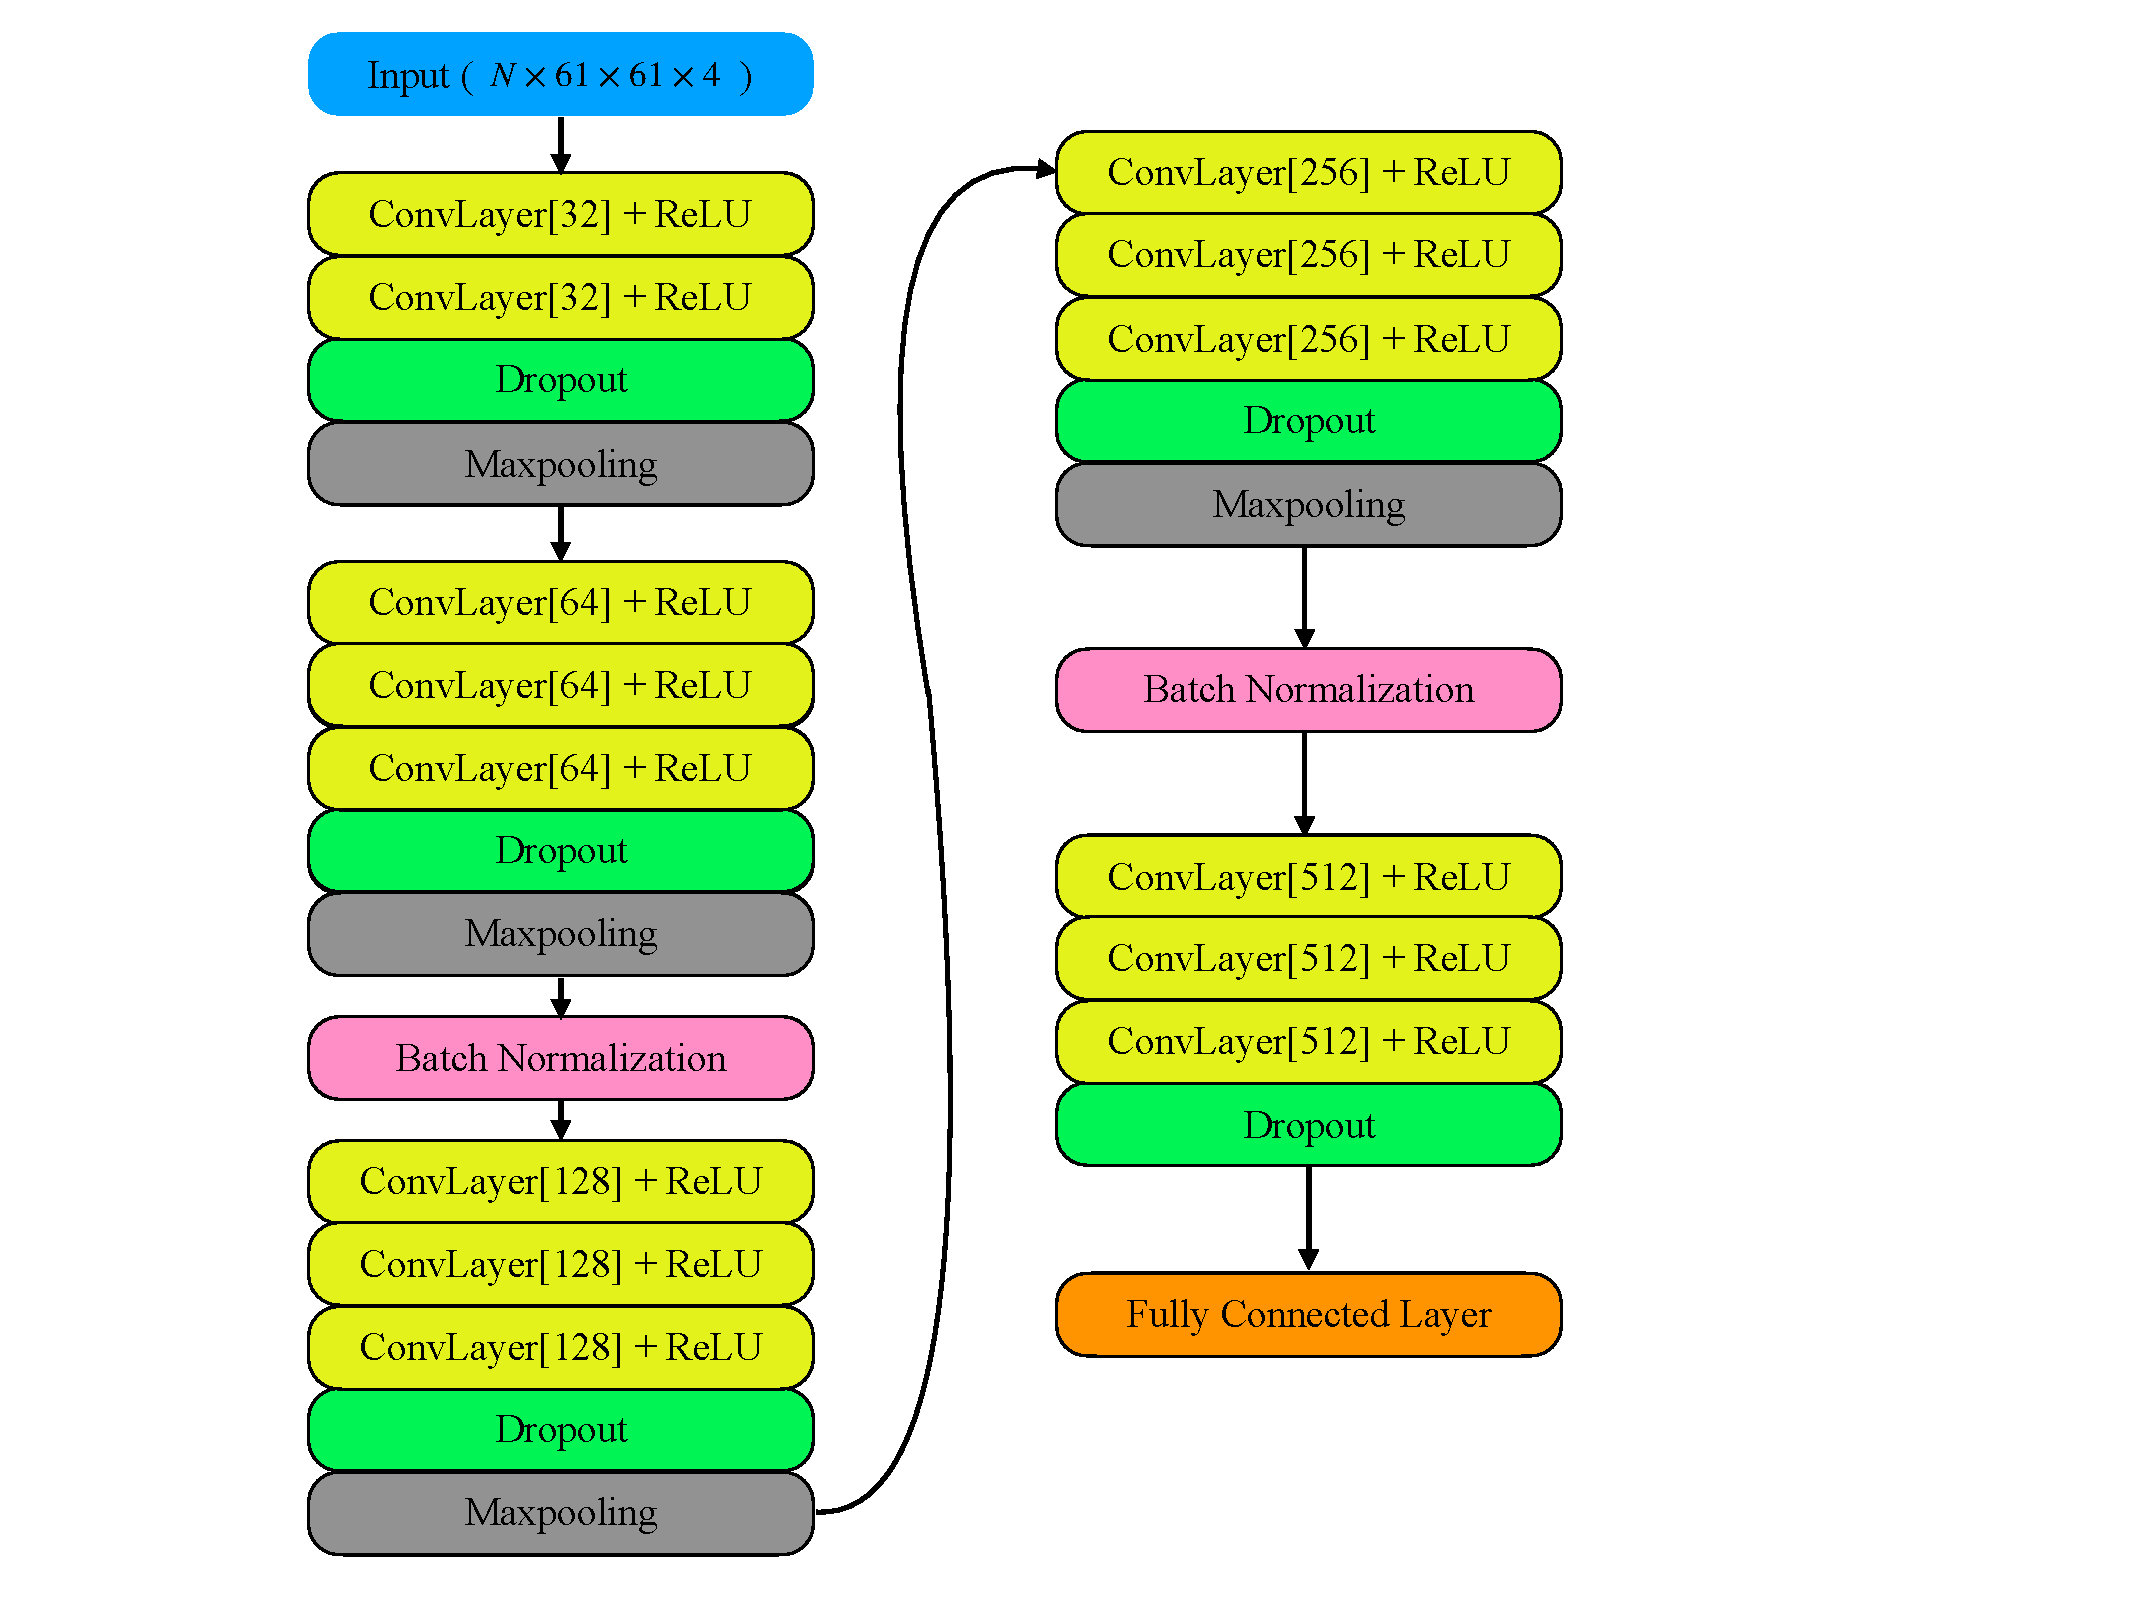
\includegraphics[width=0.5\textwidth]{../report/Figures/cnn_arc.pdf}
\end{figure}
\end{frame}

\subsection{Training Configuration}
\begin{frame}{Training Hyperparameter}
\begin{table}[h!]
        \centering
        \begin{tabular}{ l | c  }
            Hyperparameter  & Setting \\ \hline
            Activation function & ReLU \\
            Weight initilization & He normal \\
            Weight regularizer &  L2 \\
            Convolution border mode  & Same \\
            Stride & 2 \\ 
            Kernel size & $(3, 3)$ \\
            Dropout rate & $0.1$ \\
            Optimizer & SGD \\
            Initial Learning Rate & $1\times 5\times10^{-3}$ \\
            Batch Size & 200 \\
            Epoch & 1000 \\
            Validation Rate & 0.2 \\
        \end{tabular}
        \caption{Hyperparameter settings.}
        \label{table:hyper}
\end{table}
\end{frame}

\section{Results and Analysis}

\begin{frame}{Simulation Configuration}
\begin{itemize}
\item {
\textbf{World Setting}
\pause
the world box size is $30 \times 30$, and there are $50-100$ circle rigid bodies($r = 1$, all circle rigid bodies in the same size.) inside the box. Initially, the rigid circles will be located following gaussian distribution2. Then, all rigid circles will fall down by gravity.
\pause
}
\item {
\textbf{Simulation Setting}
\pause
there will be totally 600-steps simulation. For each step, $\Delta t = 0.01s$, and the number of iteration in each step will be set as fixed, 3000.
}

\end{itemize}
\end{frame}

\begin{frame}
\begin{figure}[!h]
        \centering
        \begin{subfigure}[b]{0.3\textwidth}
            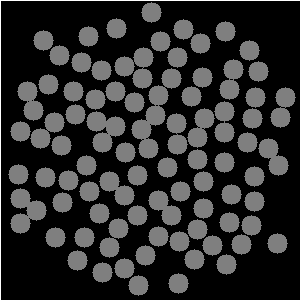
\includegraphics[width=\textwidth]{../report/Figures/sim0.png}
            \caption{Time Step=$0$}
        \end{subfigure}
        \begin{subfigure}[b]{0.3\textwidth}
            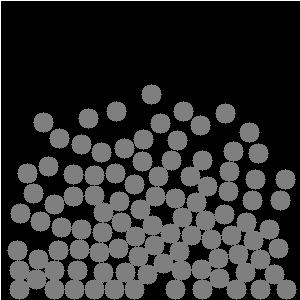
\includegraphics[width=\textwidth]{../report/Figures/sim2.png}
            \caption{Time Step=$200$}
        \end{subfigure}
        \begin{subfigure}[b]{0.3\textwidth}
            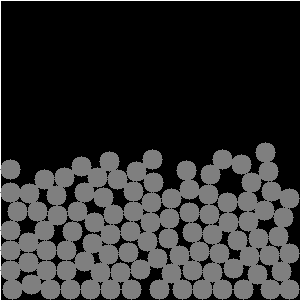
\includegraphics[width=\textwidth]{../report/Figures/sim3.png}
            \caption{Time Step=$400$}
        \end{subfigure}
        \caption{Visualization for experiment simulation}
        \label{fig:imsim}
\end{figure}
\end{frame}

\begin{frame}{Results and Analysis}{SPH parameters}
I define $\pmb{d}=(d_x, d_y)$ as grid cell size and $h$ as smoothing length.
\begin{itemize}
	\pause
        \item Since the objects are circles, $d_x = d_y = d $ 
	\pause
        \item $d$ must be less than the distance of nearest two contact points. It can be defined. $d \le r = 1$
	\pause
        \item the smooth length $h$ should be less than the minimum distance between two contact points $d$, $h \le d$  
        \pause
	\item For a given $d$, $h \ge \frac{\sqrt{2}}{2}d \approx 0.71 d$
\end{itemize}
\end{frame}

\begin{frame}{Results and Analysis}{SPH parameters(\textbf{Poly6})}
\begin{figure}[!ht]
    \centering
    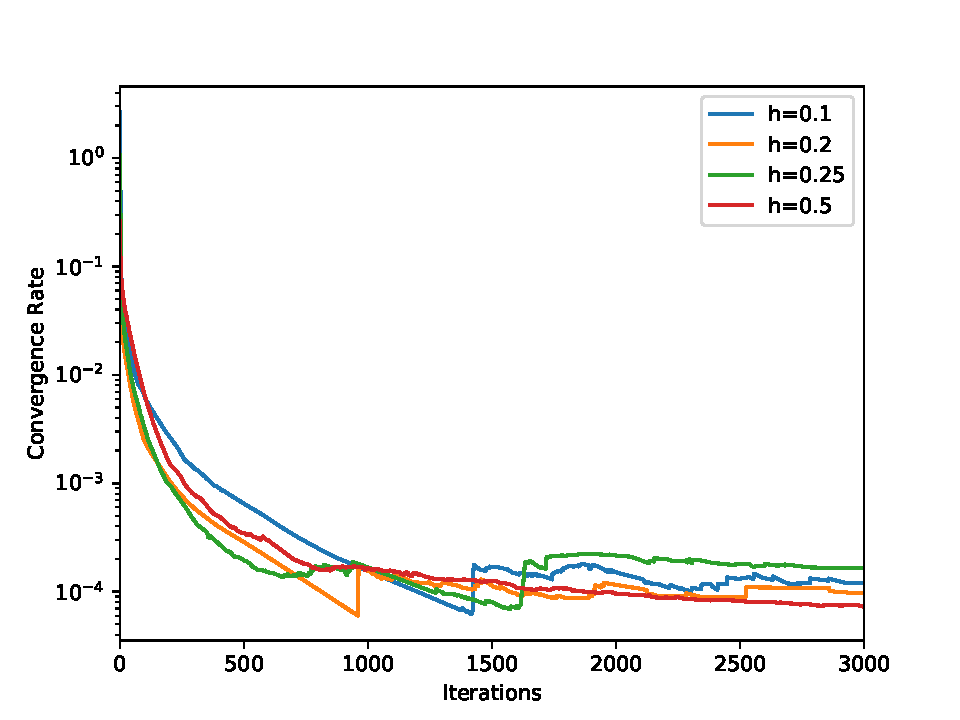
\includegraphics[scale=0.4]{../report/Figures/size25.pdf}
    \caption{The grid size $d$ is set $0.25$. $h=0.1, 0.2, 0.25, 0.5$ is tested respectively. This figure shows different coveragence rate based on different $h$ value. The kernel is \textbf{Poly6}}
\end{figure}
\end{frame}
\begin{frame}{Results and Analysis}{SPH parameters(\textbf{Poly6})}
\begin{figure}[!ht]
    \centering
    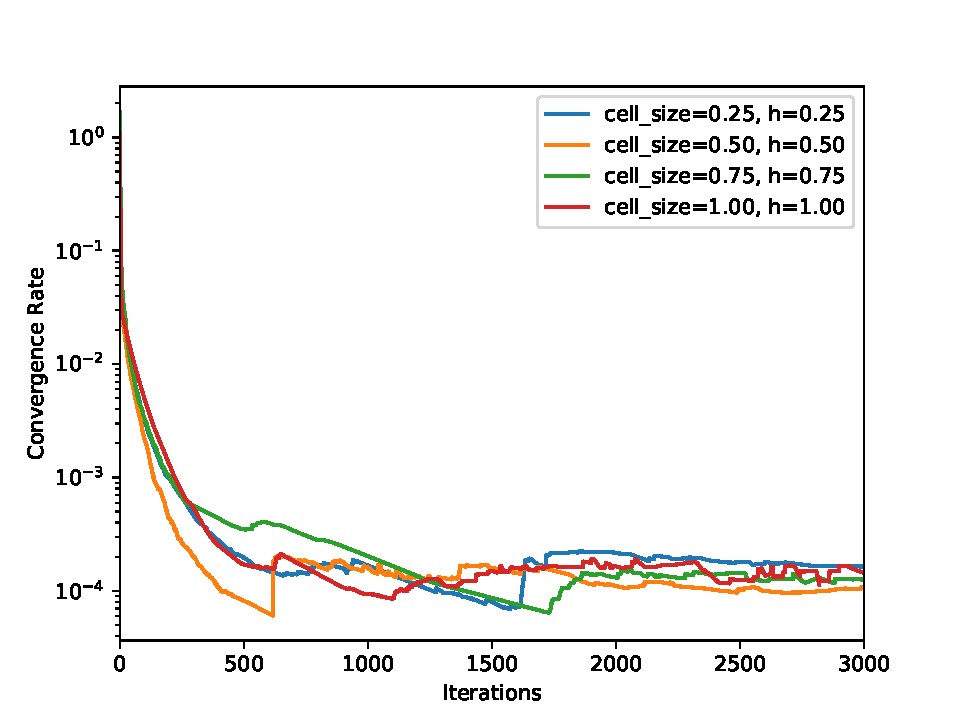
\includegraphics[scale=0.4]{../report/Figures/hd.pdf}
    \caption{Coveragence rate for different $d$ value. The kernel is \textbf{Poly6}}
\end{figure}
\end{frame}

\begin{frame}{Results and Analysis}{SPH parameters(\textbf{Spiky})}
\begin{figure}[!ht]
    \centering
    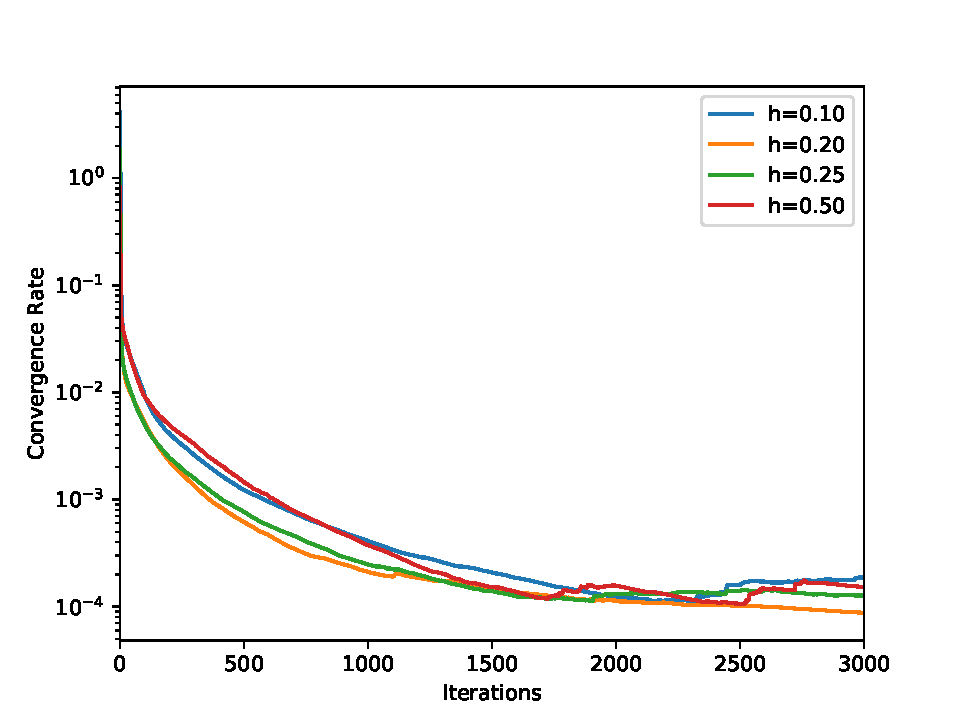
\includegraphics[scale=0.4]{../report/Figures/spiky25.pdf}
    \caption{The grid size $d$ is set $0.25$. $h=0.1, 0.2, 0.25, 0.5$ is tested respectively. This figure shows different coveragence rate based on different $h$ value. The kernel is \textbf{Spiky}}
\end{figure}
\end{frame}
\begin{frame}{Results and Analysis}{SPH parameters(\textbf{Spiky})}
\begin{figure}[!ht]
    \centering
    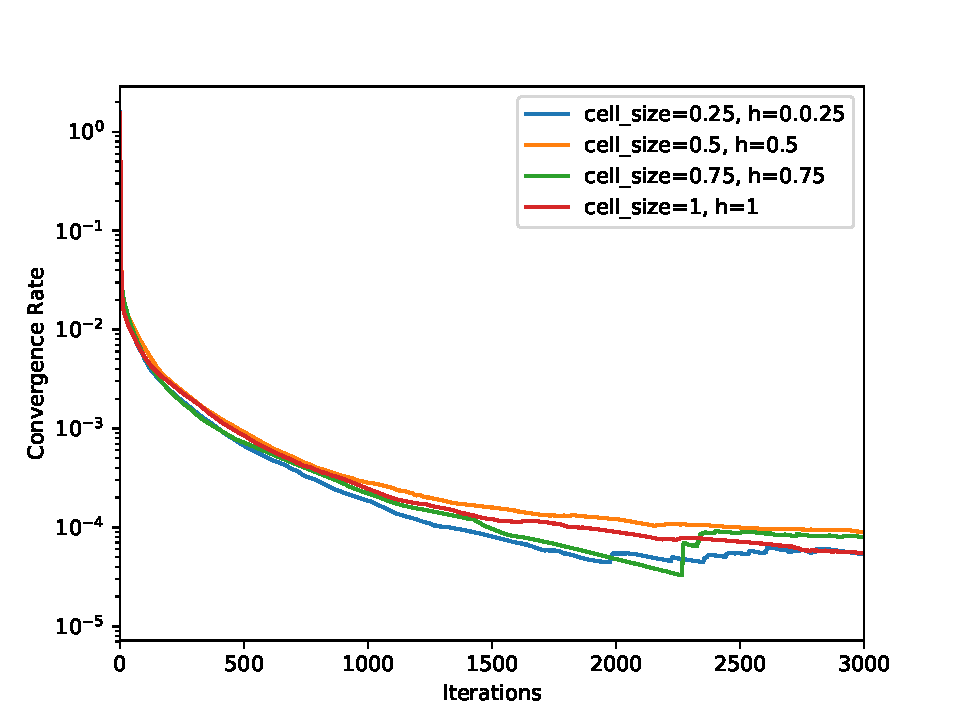
\includegraphics[scale=0.4]{../report/Figures/spikysize.pdf}
    \caption{Coveragence rate for different $d$ value. The kernel is \textbf{Spiky}}
\end{figure}
\end{frame}

\begin{frame}{Results and Analysis}{SPH parameters}
\begin{figure}[!ht]{}
        \centering
        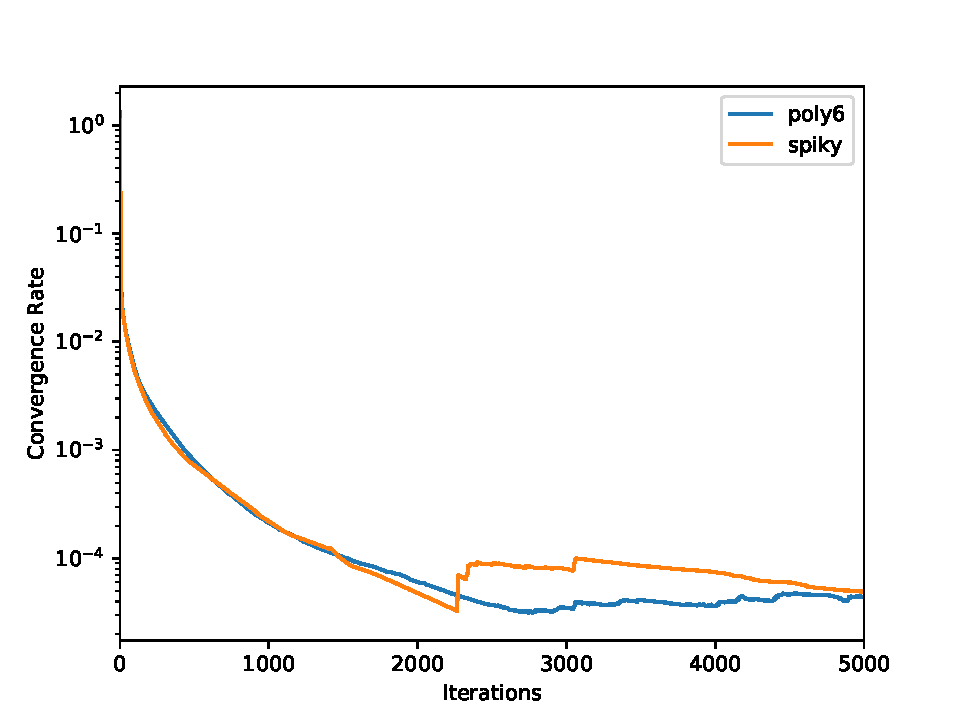
\includegraphics[scale=0.4]{../report/Figures/kerneltest.pdf}
        \caption{Coveragence rate for kernel \textbf{Poly6} anf \textbf{Spiky}. $h_\text{poly6} = d_\text{poly6} = 0.5$, while $h_\text{spiky} = d_\text{spiky} = 0.25$}
\end{figure}
\end{frame}

\begin{frame}{Results and Analysis}{SPH parameters}
\begin{figure}[!ht]
        \centering
        \includegraphics[scale=0.4]{../report/Figures/final_SPH.pdf}
        \caption{Coveragence rate for models(different initial values for $\pmb{\lambda}$).}
\end{figure}
\end{frame}
\begin{frame}{Results and Analysis}{CNN Training}
\begin{itemize}
	\pause
        \item \textbf{Input Size}, the input will be $61\times61\times4$. Since the orginal world is $30\times30$ and grid size is $d=0.5$, the generated grid would be $61\times61$. There would $4$ channels$[m, v_x, v_y, \omega]$
        \pause
	\item \textbf{Output Size}, output size depends on the label size. The orginal label image would be $[\lambda_n, \lambda_t]$, so the label image size would be $61\times61\times2$, which should be flattened as the actual training label. The label size would be $61\times 61 \times 2$
        \pause
	\item \textbf{Weights Number}, the total weights number is $64,498,866$.
	\pause
	\item \textbf{Training Environment}, GPU(\textit{GeForce GTX 1080 Ti, 11 Gbps GDDR5X memory}) held by Image Section, DIKU.
\end{itemize}
\end{frame}

\begin{frame}{Results and Analysis}{Simulation on CNN}
\begin{figure}[!h]
    \centering
    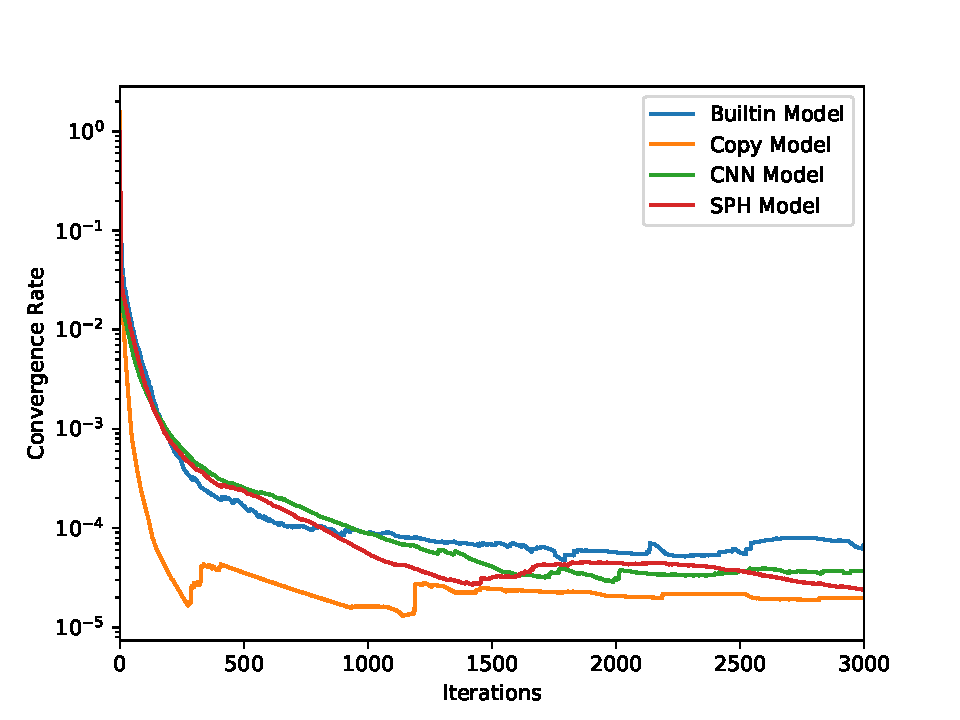
\includegraphics[scale = 0.4]{../report/Figures/cnn.pdf}
    \caption{The final result. Add the final CNN solution to compare with other methods.}
    \label{testoneworld}
\end{figure}
\end{frame}
\begin{frame}{Results and Analysis}{Simulation on CNN}
\begin{figure}[!h]
        \centering
            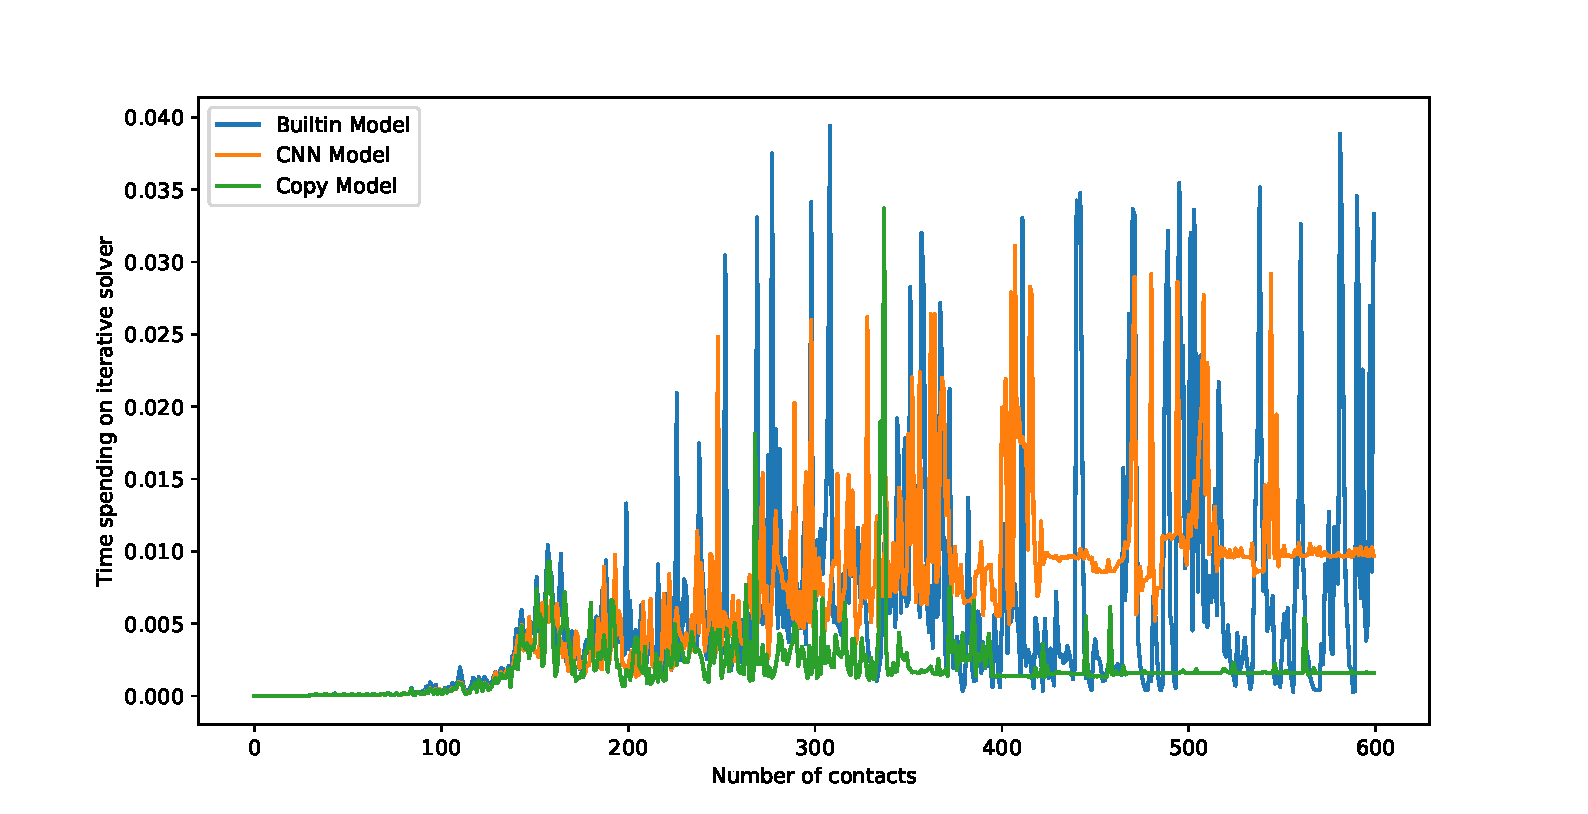
\includegraphics[scale = 0.4]{../report/Figures/cnntime}
            \caption{Time spent for contact solver iteration}
\end{figure}
\end{frame}
\begin{frame}{Results and Analysis}{Simulation on CNN}
\begin{figure}[!h]
        \centering
            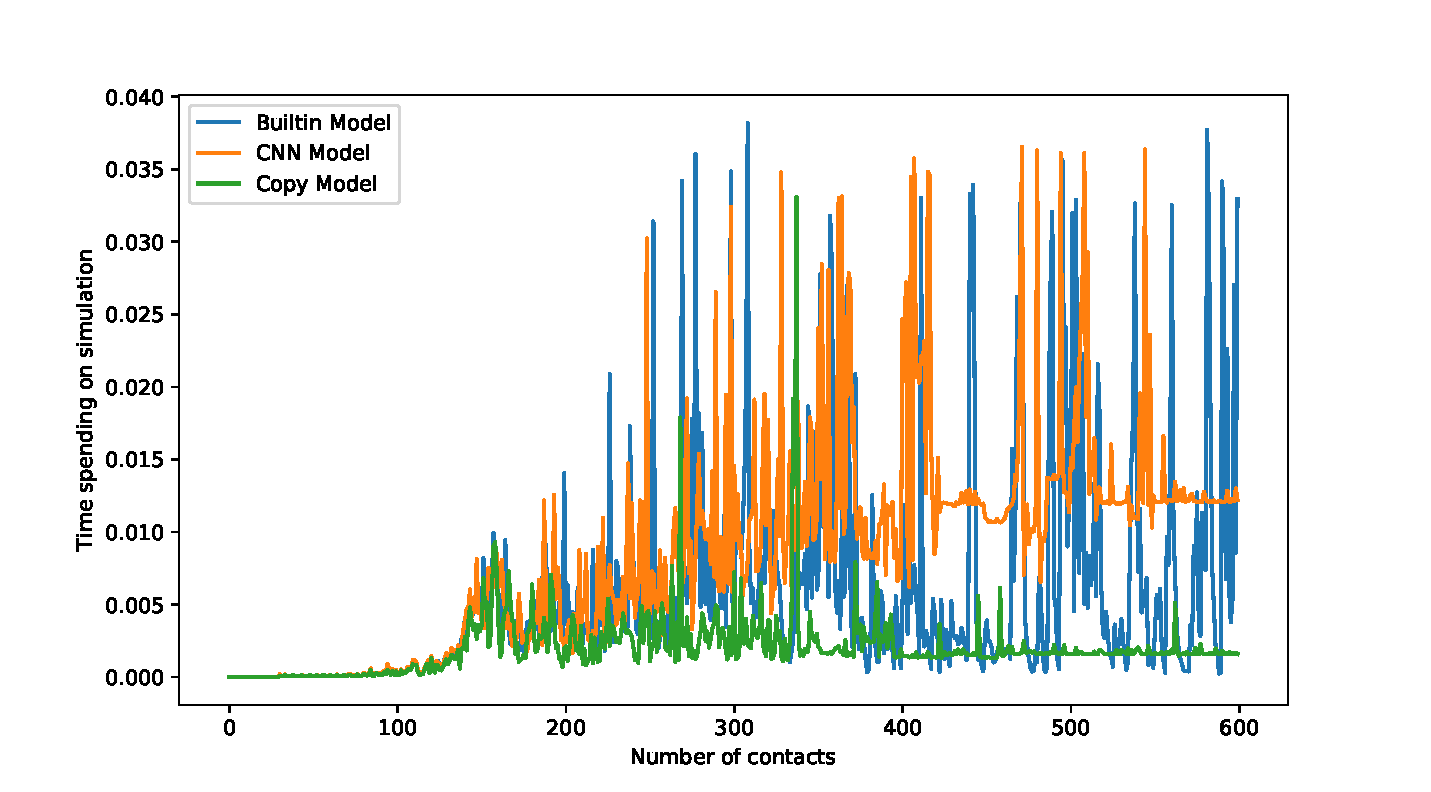
\includegraphics[scale = 0.4]{../report/Figures/cnntotal}
            \caption{Time spend for the whole contact solution(including warm starting calculation).}
\end{figure}
\end{frame}

\begin{frame}{Results and Analysis}{Conclusion}
Now, we can obtain some conclusions,
\pause
\begin{itemize}
    \item \textbf{CNN-Model} actually makes the iterative solver converge faster. But it is not a great improvement to buit-in warm starting.
    \pause
    \item \textbf{CNN-Model} performs very similar to \textbf{SPH-Model}, which means the CNN predicts contact image well.
    \pause
    \item Due to the limitation of the SPH-based method, \textbf{CNN-Model} just gets a small improvement compared with \textbf{Builtin-Model}. And it cannot perform as good as \textbf{Copy-Model}.
\end{itemize}
\end{frame}


\section{Future Work}
\begin{frame}{Future Work}
\begin{enumerate}
\item {
\textbf{Grid-Particles Method}
\pause
\begin{itemize}
\item {
\textbf{SPH}
\pause
For the SPH-based method, it is still far away from perfect. It performs not much better than warm starting. The probable attempt will including trying more new kernels, using new data and algorithm for nearest neighbor searching.
\pause
}
\item {
\textbf{Interpolation Method}
\pause
It might lose some essential informa- tion when it was interpolated back to particles. So exploring another interpolation method would be helpful to this project.
\pause
}
\end{itemize}
}

\item {
\textbf{Deep Learning Model},
\pause
More learning models can be explored, like Recurrent Neural Networks(RNN),  Long short-term memory(LSTM).
\pause
}

\item {
\textbf{More Shapes Experiments}
}
\end{enumerate}

\end{frame}


% All of the following is optional and typically not needed. 
\appendix
\section<presentation>*{\appendixname}
\subsection<presentation>*{For Further Reading}

\begin{frame}[allowframebreaks]
  \frametitle<presentation>{For Further Reading}
    
  \begin{thebibliography}{10}
    
  \beamertemplatebookbibitems
  % Start with overview books.

  \bibitem{Author1990}
    A.~Author.
    \newblock {\em Handbook of Everything}.
    \newblock Some Press, 1990.
 
    
  \beamertemplatearticlebibitems
  % Followed by interesting articles. Keep the list short. 

  \bibitem{Someone2000}
    S.~Someone.
    \newblock On this and that.
    \newblock {\em Journal of This and That}, 2(1):50--100,
    2000.
  \end{thebibliography}
\end{frame}

\end{document}



